\section{结构化控制结构}
\hfill\ctli{实验时间}{~2015~年~1~月~8~日}
\subsection*{【实验目的】}
\begin{enumerate}[topsep=0pt,partopsep=0pt,itemsep=0pt,parsep=0pt,label={\arabic*、}]
\item 掌握基本的结构化控制结构。
\item 能够熟练进行结构化编程。
\end{enumerate}
\subsection*{【实验环境】}
\MyEnvironment
\subsection*{【实验内容】}
\begin{enumerate}[topsep=0pt,partopsep=0pt,itemsep=0pt,parsep=0pt,label={\arabic*、}]
\item 编写NumberA类,实现两个整数的加减乘除运算,可以循环计算。构造函数实现两整数a,b赋值。
\item P177:5.29
\end{enumerate}

\subsection{NumberA 类}
\subsubsection*{【详细分析】}
NumberA 类设有两个成员变量存放两个操作数,提供对这两个操作数进行四则运算的方法。

主程序循环读入两个整数,进行运算并输出。
\subsubsection*{【实验源码】}
{\linespread{1}\lstinputlisting[caption={\tt exp01.cpp}]{exp03/exp01.cpp}}
\subsubsection*{【实验结果】}
\begin{figure}[htp]
\centering
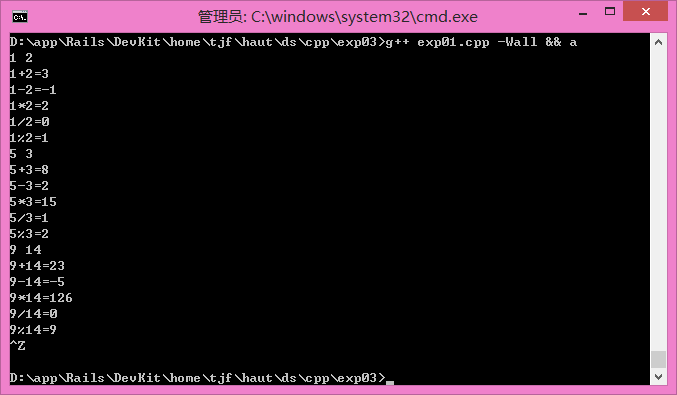
\includegraphics[width=\textwidth]{exp03/exp01.png}
\caption{\label{out03_01}NumberA 类}
\end{figure}

\subsection{Peter Minuit 问题}
\subsubsection*{【详细分析】}
复利的计算,基于课本的示例程序修改。通过在年份循环之外加上利率的循环,计算出不同利率下的本息变化。
\subsubsection*{【实验源码】}
{\linespread{1}\lstinputlisting[caption={\tt exp03.cpp}]{exp03/exp02.cpp}}
\subsubsection*{【实验结果】}
\begin{figure}[htp]
\centering
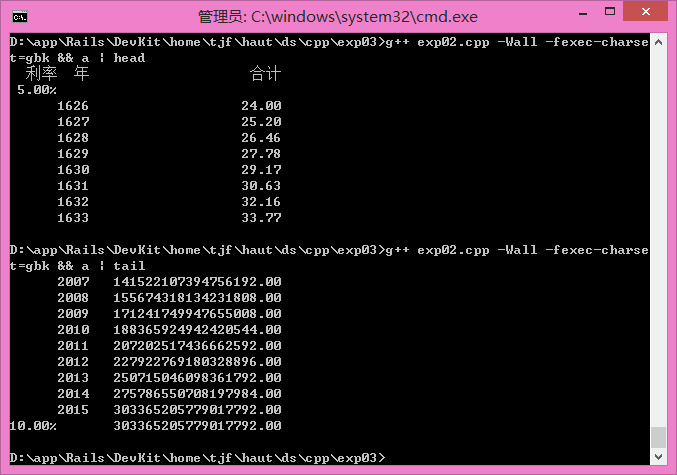
\includegraphics[width=\textwidth]{exp03/exp02.png}
\caption{\label{out03_02}Peter Minuit 问题}
\end{figure}
由于程序输出非常多,图\ref{out03_02} 只给出了程序的前后十行的输出。

\subsection*{【实验体会】}
这次实验主要是对控制语句的应用。C++ 的流程控制语句与 C 一脉相承,并没有太大差别。对于循环语句,三大循环语句其实是可以互相转换的,虽然如此,也要视场合选用合适的语句,不能因为 for 语句的强大而滥用,导致代码变得难以理解。分支语句也是以 if/else if/else 为主的。总之基本流程就是这么多了,搞清楚其中的逻辑关系和嵌套、作用域就好。
